\startslide{Presentation Outline}

\begin{cenumerate}
\item Motivations, design overview
\item Technical details
\begin{citemize}
\item Language design 
\item Formal foundations
\end{citemize}
\item Language implementation and application
\end{cenumerate}

\stopslide

\startslide{Presentation Outline}

\begin{cenumerate}
\item \cemph{Motivations, design overview}
\item Technical details
\begin{citemize}
\item Language design 
\item Formal foundations
\end{citemize}
\item Language implementation and application
\end{cenumerate}

\stopslide

\startslide{The Problem Setting: Embedded Sensor Networks}

%\includegraphics{sagehen-deploy}

\begin{citemize}
\item Distributed data-gathering systems for earth and agricultural sciences.
\item At UVM, focus on sytems alpine snow hydrology.
\begin{citemize}
\item Deployments in California, New Hampshire, Arctic Norway.
\end{citemize}
\end{citemize}
\stopslide

\startslide{The Problem Setting: Embedded Sensor Networks}

\begin{center}
%\includegraphics[scale=.3]{motes}
\end{center}

\begin{citemize}
\item \cemph{Mote} computation and communications platform.
\item Crossbow TelosB: 4MHz, 10KB RAM, 48K ROM.
\end{citemize}
\stopslide

\startslide{Unique Challenges of Programming WSNs}

\begin{citemize}
\item Heavily resource constrained-- RAM, ROM, clock cycles, power.
\item ... yet complex, distributed algorithms
\begin{citemize}
\item ``True'' specification at \cemph{macro} (network) level.
\end{citemize}
\end{citemize}
State of the art:
\begin{citemize}
\item TinyOS and nesC programming: optimized for efficiency, widely used.
\item Various \cemph{macroprogramming} proposals, but mostly ad hoc 
node level programming techniques in practice.
\end{citemize}
\stopslide

\startslide{Program Staging aka Metaprogramming aka Partial Evaluation}

\begin{citemize}
\item \cemph{Specialization}: given a program template define algorithms that 
automatically make applications more compact and efficient.
\item Metaprogramming allows macroprogramming of device level code.
\end{citemize}

\stopslide

\startslide{How Would It Be Used?}

\vspace{.4in}
\begin{center}
%\includegraphics{lab}
\end{center}

In the lab.
\begin{citemize}
\item Device code specialized prior to deployment.
\item Application: key distribution for resource authorization.
\end{citemize}

\stopslide

\startslide{How Would It Be Used?}


$$
\begin{array}{l@{\qquad}l}
%\includegraphics[scale=.08]{mammoth-gateway}
&
%\includegraphics[scale=.15]{gateway}  
\end{array}
$$

On a deployed \cemph{hub}.
\begin{citemize}
\item Gateway devices higher powered, full Linux box.
\item Application: \emph{backcasting}, dynamic refinement of sampling models.
\emph{in situ}.
\end{citemize}

\stopslide

\startslide{Our Approach}

\begin{citemize}
\item \cemph{Lightweight macroprogramming}. Scala at metalevel, nesC 
residuum.
\item Technical features: type specialization, process separation.
\item \cemph{Cross-stage type safety}: type checking at Scala level ensures
type safety of nesC residuum.
\item \cemph{Well-founded language design}.
\end{citemize}

\stopslide

\startslide{Contrast with Related Work}

\cemph{Flask}: Mainland, Morrisett, Welch 2008.
\begin{citemize}
\item Macroprogramming functional language.
\item Staging techniques generate device-level code from macroprogram.
\end{citemize}
In our work:
\begin{citemize}
\item Total programmer control over device level code (efficiency over expressivity).
\item Accessible imperative (vs.~declarative) model.
\item Cross-stage type safety.
\end{citemize}

\stopslide

\startslide{Presentation Outline}

\begin{cenumerate}
\item Motivations, design overview
\item \cemph{Technical details}
\begin{citemize}
\item \cemph{Language design} 
\item Formal foundations
\end{citemize}
\item Language implementation and application
\end{cenumerate}

\stopslide

\startslide{Language Model and Scope}

In intended application space, computational model includes network 
communication:
\begin{citemize}
\item Obtain environmental information from network
\item Deployment of specialized code
\end{citemize}
Existing protocols and libraries address these. \cemph{We focus on novel
program staging feature semantics and typing}.
%:
%\begin{citemize}
%\item TinyOS JVM libraries for communication of small values
%\item Deluge for dissemination of large values (OS images)
%\end{citemize}
%Focus on semantics and typing for program staging features.
\stopslide

\startslide{Two Program Stages: Scalaness/nesT}
Language model incorporates two distinct program stages.
\begin{citemize}
\item \cemph{First Stage}: for execution in lab or 
on hub device.
\begin{citemize}
\item Written in a Scala variant (\cemph{Scalaness}).
\item Code-as-value realized as first class TinyOS modules.
\item Operations on module datatype allow program specialization.
\end{citemize}
\item \cemph{Second Stage}: for deployment 
and execution on network devices.
\begin{citemize}
\item Written in type safe variant of nesC (\cemph{nesT}).
\item Supports integration of TinyOS libraries.
\end{citemize}
\end{citemize}

\stopslide

\startslide{Example: Specializing the Radio Stack}

TinyOS radio stack allows static configuration of message size.

Allow specialization of radio stack based on application context:
\begin{citemize}
 \item \cemph{Length} of message payload.
 \item \cemph{Type} of message header (address size).
\end{citemize}
Potentially \emph{big win}: power consumption in many applications
dominated by messaging overhead.
\stopslide

\startslide{Scalaness/nesT Example}

$$
\begin{array}{rcl}
\texttt{messageT} &\defeq& \texttt{\{src:X; dest:X; data:uint8[\,]\}} \\[5mm]
\texttt{radioT} &\defeq& \texttt{<mt $\subtype$ messageT[uint], paysize:uint>} \\
 & & \texttt{\{\ export\  error\_t\ radio (adt)\ \}}\\[5mm]
%\texttt{senderT} &\defeq& \texttt{< > \{\ export\  error\_t\ send (messageT)\ \}}\\[2mm]
\end{array} 
$$
$$
\begin{array}{lcl}
\texttt{sendC} & = & \texttt{<adt $\subtype$ uint>}\\
&& \texttt{\{ import error\_t radio(messageT[adt]);}\\
&& \texttt{\phantom{\{ }export error\_t send (s:adt, d:adt, uint8[] data)}\\
&& \texttt{\phantom{\{ }\{ radio(\{src = s, dest = d, data = data\}); \}\ \}}\\[10mm]
\multicolumn{3}{l}{\texttt{def sendSpecialize(nmax:uint16, paysize:uint, radioC:radioT)}}\\
\{\\
\multicolumn{3}{l}{\quad \texttt{typedef adt $\subtype$ uint16 = if (nmax <= 256) uint8 else uint16;}}\\
\multicolumn{3}{l}{\quad \texttt{sendC<adt> $\ltimes$ radioC<messageT[adt], paysize>;}}\\
\}
\end{array}
$$

\stopslide

\startslide{Syntactic Sugar for Presentation}

$$
\begin{array}{rcl}
\texttt{\color{red}{messageT}} &\color{red}{\defeq}& \texttt{\color{red}{\{src:X; dest:X; data:uint8[\,]\}}} \\[5mm]
\texttt{radioT} &\defeq& \texttt{<mt $\subtype$ messageT[uint], paysize:uint>} \\
 & & \texttt{\{\ export\  error\_t\ radio (adt)\ \}}\\[5mm]
%\texttt{senderT} &\defeq& \texttt{< > \{\ export\  error\_t\ send (messageT)\ \}}\\[2mm]
\end{array} 
$$
$$
\begin{array}{lcl}
\texttt{sendC} & = & \texttt{<adt $\subtype$ uint>}\\
&& \texttt{\{ import error\_t radio(messageT[adt]);}\\
&& \texttt{\phantom{\{ }export error\_t send (s:adt, d:adt, uint8[] data)}\\
&& \texttt{\phantom{\{ }\{ radio(\{src = s, dest = d, data = data\}); \}\ \}}\\[10mm]
\multicolumn{3}{l}{\texttt{def sendSpecialize(nmax:uint16, paysize:uint, radioC:radioT)}}\\
\{\\
\multicolumn{3}{l}{\quad \texttt{typedef adt $\subtype$ uint16 = if (nmax <= 256) uint8 else uint16;}}\\
\multicolumn{3}{l}{\quad \texttt{sendC<adt> $\ltimes$ radioC<messageT[adt], paysize>;}}\\
\}
\end{array}
$$

\stopslide

\startslide{Scalaness/nesT Example: nesT Module Definitions}

$$
\begin{array}{rcl}
\texttt{messageT} &\defeq& \texttt{\{src:X; dest:X; data:uint8[\,]\}} \\[5mm]
\texttt{\color{red}{radioT}} &\color{red}{\defeq}& \texttt{\color{red}{<mt $\subtype$ messageT[uint], paysize:uint>}} \\
 & & \texttt{\color{red}{\{\ export\  error\_t\ radio (adt)\ \}}}\\[5mm]
%\texttt{senderT} &\defeq& \texttt{< > \{\ export\  error\_t\ send (messageT)\ \}}\\[2mm]
\end{array} 
$$
$$
\begin{array}{lcl}
\texttt{\color{red}{sendC}} & \color{red}{=} & \texttt{\color{red}{<adt $\subtype$ uint>}}\\
&& \texttt{\color{red}{\{ import error\_t radio(messageT[adt]);}}\\
&& \texttt{\phantom{\{ }\color{red}{export error\_t send (s:adt, d:adt, uint8[] data)}}\\
&& \texttt{\phantom{\{ }\color{red}{\{ radio(\{src = s, dest = d, data = data\}); \}\ \}}}\\[10mm]
\multicolumn{3}{l}{\texttt{def sendSpecialize(nmax:uint16, paysize:uint, radioC:radioT)}}\\
\{\\
\multicolumn{3}{l}{\quad \texttt{typedef adt $\subtype$ uint16 = if (nmax <= 256) uint8 else uint16;}}\\
\multicolumn{3}{l}{\quad \texttt{sendC<adt> $\ltimes$ radioC<messageT[adt], paysize>;}}\\
\}
\end{array}
$$

\stopslide

\startslide{Scalaness/nesT Example: First Class Modules}

$$
\begin{array}{rcl}
\texttt{messageT} &\defeq& \texttt{\{src:X; dest:X; data:uint8[\,]\}} \\[5mm]
\texttt{radioT} &\defeq& \texttt{<mt $\subtype$ messageT[uint], paysize:uint>} \\
 & & \texttt{\{\ export\  error\_t\ radio (adt)\ \}}\\[5mm]
%\texttt{senderT} &\defeq& \texttt{< > \{\ export\  error\_t\ send (messageT)\ \}}\\[2mm]
\end{array} 
$$
$$
\begin{array}{lcl}
\texttt{sendC} & = & \texttt{<adt $\subtype$ uint>}\\
&& \texttt{\{ import error\_t radio(messageT[adt]);}\\
&& \texttt{\phantom{\{ }export error\_t send (s:adt, d:adt, uint8[] data)}\\
&& \texttt{\phantom{\{ }\{ radio(\{src = s, dest = d, data = data\}); \}\ \}}\\[10mm]
\multicolumn{3}{l}{\texttt{def sendSpecialize(nmax:uint16, paysize:uint, \color{red}{radioC:radioT})}}\\
\{\\
\multicolumn{3}{l}{\quad \texttt{typedef adt $\subtype$ uint16 = if (nmax <= 256) uint8 else uint16;}}\\
\multicolumn{3}{l}{\quad \texttt{sendC<adt> $\ltimes$ radioC<messageT[adt], paysize>;}}\\
\}
\end{array}
$$

\stopslide

\startslide{Module Instantiation and Wiring}

$$
\begin{array}{rcl}
\texttt{messageT} &\defeq& \texttt{\{src:X; dest:X; data:uint8[\,]\}} \\[5mm]
\texttt{radioT} &\defeq& \texttt{<mt $\subtype$ messageT[uint], paysize:uint>} \\
 & & \texttt{\{\ export\  error\_t\ radio (adt)\ \}}\\[5mm]
%\texttt{senderT} &\defeq& \texttt{< > \{\ export\  error\_t\ send (messageT)\ \}}\\[2mm]
\end{array} 
$$
$$
\begin{array}{lcl}
\texttt{sendC} & = & \texttt{<adt $\subtype$ uint>}\\
&& \texttt{\{ import error\_t radio(messageT[adt]);}\\
&& \texttt{\phantom{\{ }export error\_t send (s:adt, d:adt, uint8[] data)}\\
&& \texttt{\phantom{\{ }\{ radio(\{src = s, dest = d, data = data\}); \}\ \}}\\[10mm]
\multicolumn{3}{l}{\texttt{def sendSpecialize(nmax:uint16, paysize:uint, radioC:radioT)}}\\
\{\\
\multicolumn{3}{l}{\quad \texttt{typedef adt $\subtype$ uint16 = if (nmax <= 256) uint8 else uint16;}}\\
\multicolumn{3}{l}{\quad \texttt{\color{red}{sendC<adt> $\ltimes$ radioC<messageT[adt], paysize>;}}}\\
\}
\end{array}
$$

\stopslide

\startslide{Scalaness/nesT Example: Dynamic Type Construction}

$$
\begin{array}{rcl}
\texttt{messageT} &\defeq& \texttt{\{src:X; dest:X; data:uint8[\,]\}} \\[5mm]
\texttt{radioT} &\defeq& \texttt{<mt $\subtype$ messageT[uint], paysize:uint>} \\
 & & \texttt{\{\ export\  error\_t\ radio (adt)\ \}}\\[5mm]
%\texttt{senderT} &\defeq& \texttt{< > \{\ export\  error\_t\ send (messageT)\ \}}\\[2mm]
\end{array} 
$$
$$
\begin{array}{lcl}
\texttt{sendC} & = & \texttt{<adt $\subtype$ uint>}\\
&& \texttt{\{ import error\_t radio(messageT[adt]);}\\
&& \texttt{\phantom{\{ }export error\_t send (s:adt, d:adt, uint8[] data)}\\
&& \texttt{\phantom{\{ }\{ radio(\{src = s, dest = d, data = data\}); \}\ \}}\\[10mm]
\multicolumn{3}{l}{\texttt{def sendSpecialize(nmax:uint16, paysize:uint, radioC:radioT)}}\\
\{\\
\multicolumn{3}{l}{\quad \texttt{\color{red}{typedef adt $\subtype$ uint16 = if (nmax <= 256) uint8 else uint16;}}}\\
\multicolumn{3}{l}{\quad \texttt{sendC<{\color{red}adt}> $\ltimes$ radioC<messageT[{\color{red}adt}], paysize>;}}\\
\}
\end{array}
$$

\stopslide

\startslide{Well-Founded Semantics and Typing}  

Complex interaction of many elements. Module composition semantic challenges:
\begin{citemize}
\item Migration of values and types across stages.
\begin{citemize}
\item Migrating \cemph{values may contain references}.
\end{citemize}
\end{citemize}
Module composition typing challenges:
\begin{citemize}
\item Operations should preserve typeability of module components (\cemph{cross-stage type
safety}).
\item Type discipline over migrating values-- enforce \cemph{process separation}.
\item Static module types may be \cemph{abstract} (up to subtyping bounds) wrt 
dynamically \cemph{constructed types}.
\end{citemize}

\stopslide

\startslide{Presentation Outline}

\begin{cenumerate}
\item Motivations, design overview
\item \cemph{Technical details}
\begin{citemize}
\item Language design 
\item \cemph{Formal foundations}
\end{citemize}
\item Language implementation and application
\end{cenumerate}

\stopslide

\startslide{\fml\ Foundations}

The \fml\ language\footnote{\cref{Yu David Liu, Christian Skalka, and Scott Smith. Type-Specialized Staged Programming with Process Separation. Journal of Higher Order and Symbolic Computation, 24(4):341-385, 2012.}} was developed to study these elements at a foundational level.
\begin{citemize}
\item Comprises $F_{\le}$.
\item MetaML-like syntax and semantics, but novel features to moderate 
interactions between separate process spaces.
\item Resricted form of type construction (not full $\lambda_\omega$).
\item Formal metatheory includes cross-stage type safety-- residue of  
partial evaluation of well-typed code is guaranteed to be well-typed.
\end{citemize}

\stopslide

\startslide{The Model of a Module}

The essence of a nesT module definition:
{\Large
$$
\lambda x : \tau_1 . \Lambda t \subtype \tau_2 . \langle e \rangle
$$
}
\begin{citemize}
\item $\langle e \rangle$ is code-as-value (the ``module definition'').
\item $\lambda$ binds ``value parameter''.
\item $\Lambda$ binds ``type parameter'', with type bound.
\item If $x$ is free in $e$, then $\tau_1 = \langle \tau \rangle$. \cemph{The stage levels must match}.
\end{citemize}
\stopslide

\startslide{The Model of Module Instantiation}

The essence of a Scalaness/nesT module instantiation:
{\Large
$$
(\lambda x : \tau_1 . \Lambda t \subtype \tau_2 . \langle e \rangle)(\mathrm{lift}\ v) \tau
$$
}
\begin{citemize}
\item Value $v$ must be explicitly ``lifted'' to next stage.
\begin{citemize}
\item Only way for values to migrate across stages, no free variable capture as in 
MetaML.
\item Lifting enforces serialization (implicit lifting in Scalaness).
\item Enforced by the type system: require that $\tau_1 = 
\langle \tau' \rangle$ and $v : \tau'$.
\end{citemize}
\end{citemize}
\stopslide

\startslide{Type Construction and Escape}

A $\mathrm{tlet}$ binding mechanism allows construction of types:
{\large
$$
\mathrm{tlet\ } t \subtype \mathrm{uint16} = \metaite{e}{\mathrm{uint8}}{\mathrm{uint16}} 
\mathrm{\ in\ }(\lambda x : t . x)\\
$$
}
\begin{citemize}
\item Restriction: only concrete types are values, no higher-order type constructors.
\item Dynamically constructed types may escape their scope.
\end{citemize}

\stopslide

\startslide{Type Construction and Escape}

We introduce an \cemph{$\exists$ type binder} for typing constructed type escape:
{\large
\begin{eqnarray*}
&\mathrm{tlet\ } t \subtype \mathrm{uint16} = \metaite{e}{\mathrm{uint8}}{\mathrm{uint16}} 
\mathrm{\ in\ }(\lambda x : t . x)\\
&: \\
&\exists t \subtype \mathrm{uint16} . t \rightarrow t
\end{eqnarray*}
}
\cemph{Execution obtains a \emph{refinement} of the type}; assuming $e \rightarrow^* \mathrm{true}$:
{\large
$$
\ldots \rightarrow^* (\lambda x : \mathrm{uint8} . x) 
\qquad \text{where} \ \ (\lambda x : \mathrm{uint8} . x) : \mathrm{uint8} \rightarrow
 \mathrm{uint8}
$$
}
Cross-stage type safety does not interfere with code type specialization.
\stopslide

\startslide{$\exists$ Type?}

Usage of $\exists$ type is non-standard.
\begin{citemize}
\item No pack, unpack rules.
\end{citemize}
But several appealing features of the approach:
\begin{citemize}
\item Sound typing $\Gamma, \Delta \vdash e : \tau$ must \cemph{encapsulate} the definition of constructed types.

{\small
\begin{mathpar}
\inferrule[TLet]
{
\stjudge{\Gamma}{\Delta}{e}{\typet[\sigma]}\\
%\Delta \vdash \tau'' \subtype \tau'\\
\stjudge{\Gamma}{\Delta; t \subtype \sigma}{e'}{\tau}
}
{\stjudge{\Gamma}{\Delta}{\tlet{t \subtype \sigma}{e}{e'}}
  {\exists t \subtype \sigma . \tau}}

\inferrule[$\exists$-E]{\Gamma, \Delta; \vdash e : \exists t \subtype \tau' . \tau
  \\  t \not\in \Delta, \Gamma}{
 \Gamma, \Delta; t\subtype \tau' \vdash e : \tau}
\end{mathpar}
}

where $\Delta$ subtyping coercions, $\Gamma$ free variable typings, $t$ in \TirName{TLet}
has \emph{eigenvariable} interpretation.
\end{citemize}

\stopslide

\startslide{$\exists$ Type?}

Bounded $\exists$ type form well-studied, esp.~Ghelli and Pierce 1998:
\begin{citemize}
\item Crucial elements of type checking in $F_\le$ (\emph{promotion}).
\item \cemph{Decidable} subtyping relation, with algorithm.
\begin{citemize}
 \item Covariant $\exists$ type bounds sound but undecidable.
 \item Invariant $\exists$ bounds decidable. 
\end{citemize}
\end{citemize}

\stopslide

\startslide{Putting it together in Scalaness}
$$
\jmodt{\Delta_1}{\margs{\Delta_2, \Gamma}\lc 
  \imports; \exportsty \rc}
$$
Module type form, where:
\begin{citemize}
\item $\Delta_1$ bounds of types constructed externally to the module
\item $\Delta_2$, $\Gamma$ type parameter bounds and term parameter types
\item $\imports$, $\exports$ import and export type signatures
\end{citemize}
$$
\inferrule[ModInstT]
{\Gamma \vdash \tt{e} : \jmodt{\varnothing}{\margs{\vect{t} \subtype \vect{\t}_1; 
 \vect{x} : \vect{\t}_2} \lc 
  \imports; \exportsty \rc}\\
 \Gamma \vdash \ttvec{e}_1 : \jinst{Type}{\ttvec{T}_1}\\
 \Gamma \vdash \ttvec{e}_2 : \ttvec{T}_2 \\
 \vdash \codt{\ttvec{T}_1} \subtype \vect{\t}_1\\
 \vdash \codt{\ttvec{T}_2} \subtype \vect{\t}_2
}
{\Gamma \vdash \jinst{e}{\ttvec{e}_1; \ttvec{e}_2} : \jmodt{\vect{t}\subtype \codt{\ttvec{T}_1}}{\margs{} \lc
  \imports; \exportsty \rc} }
$$

$\codt{T}$ is syntactic type transformation/interpretation (Scalaness to nesT).
\stopslide

\startslide{Presentation Outline}

\begin{cenumerate}
\item Motivations, design overview
\item Technical details
\begin{citemize}
\item Language design 
\item Formal foundations
\end{citemize}
\item \cemph{Language implementation and application}
\end{cenumerate}

\stopslide

\startslide{Implementation}
Scalaness/nesT has been implemented.
\begin{citemize}
\item nesT defined as restricted subset of nesC, compiled as nesC with some 
rewriting (e.g.~array bounds checks).
\item Scalaness defined by extension to the Scala compiler and plugin architecture.
\item Type checking extends Scala type checker with module types, module operation 
typings, nesT type checking. 
\end{citemize}
Github repository at \url{http://tinyurl.com/a85z8cu}.
\stopslide

\startslide{Implementation}


\hspace*{.6in}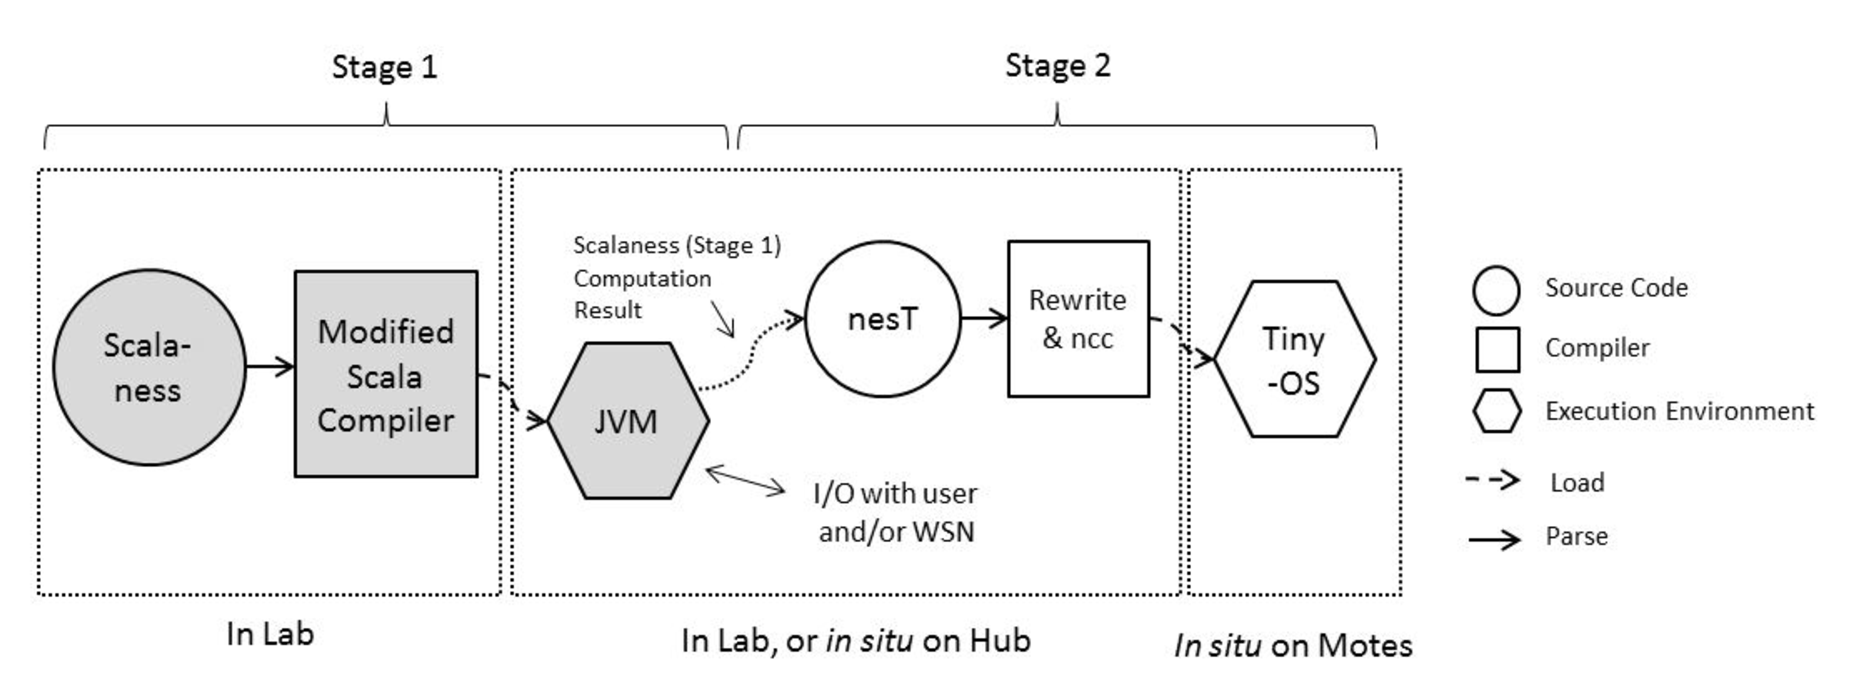
\includegraphics{scalaness}

\stopslide

\startslide{Application: WSN Session Key Negotiation}

Currently studying authorization scheme for WSNs.
\begin{citemize}
\item WSN may comprise interacting security domains with different credentials
and policies.
\item Symmetric keys provide efficient foundation for securing access.
\item Public keys allow symmetric key negotiation (Diffie-Hellman) in ``open world''
model.
\end{citemize}
Public key signature verification wildly expensive in WSNs; around 90 seconds
on Crossbow TelosB.

\cemph{Refactor session key negotiation and authorized access into 
different stages.}
\stopslide
%
%\startslide{Application: WSN Session Key Negotiation}
%
%Use Scalaness/nesT to orchestrate more efficient key negotiation:
%\begin{citemize}
%\item 
%\item Key negotiation performed over on communicating high-powered 
%hubs in first stage code.
%\item Specialize second stage code with negotiated key material, deploy 
%to WSN nodes for authorized resource access.
%\end{citemize}
%\stopslide

\startslide{Application: WSN Session Key Negotiation}

\hspace*{.6in}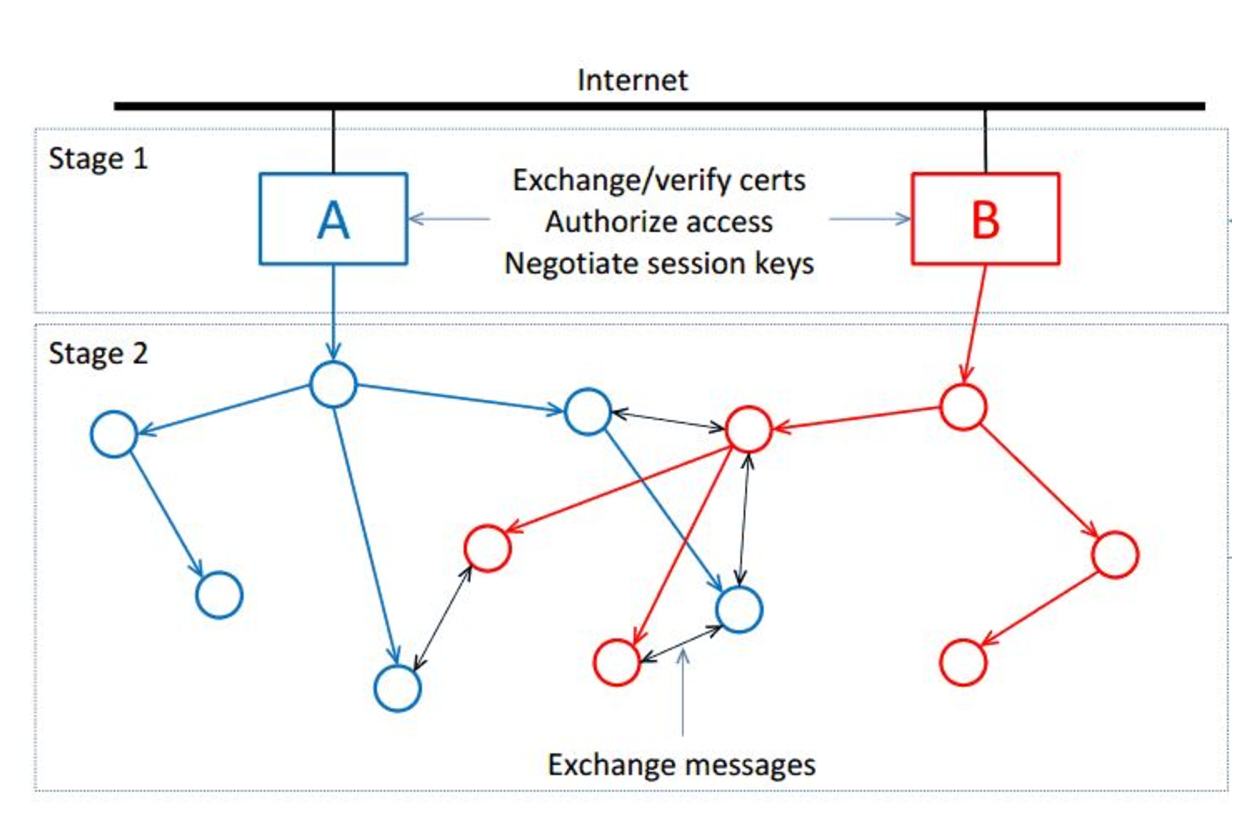
\includegraphics{spartanrpc}

Decreases WSN computational overhead, RAM and ROM consumption. 
\stopslide

\startslide{Future Work}

\begin{citemize}
\item Clarifying ``middle ground'' between langage borders, syntactic transformations.
\item Incorporating network communication. 
\item Other applications: backcasting and evolving control.
\end{citemize}

\stopslide

\startslide{Questions?}

\stopslide
